
\chapter{Úvod}
V současném světě je stále více rozšířeným užití biometrie jako součásti bezpečnostních mechanismů. Jednou z nejrozšířenějších biometrik je otisk prstu. Pro snímání by měly být zaručeny ideální podmínky, avšak se jedná o nesplnitelný úkol v běžném nasazení. Snímky získané ze senzoru mohou být nekvalitní, mohou obsahovat nečistoty, které dále komplikují proces rozpoznávání. Vysoké procento populace trpí kožními onemocněními. Mnohá onemocnění jsou široce rozšířená -- např. atopický ekzém nebo bradavice. U některých z~onemocnění (např. bradavice) je jejich vliv na rozpoznávání nižší, protože papilární linie jsou zachovány v nepostiženém místě otisku prstu, u tolik rozšířeného atopického ekzému však jsou ve vážnějších podobách papilární linie těžko rozpoznatelné. Potenciální detektor a klasifikátor těchto onemocnění by mohl odhalit možná postižení uživatele využívající biometrický systém.

Problematika detekce a klasifikace pro rozličné typy objektů je stále jedním z předních témat současnosti. Techniky, které kdysi spíše využívaly ruční extrakci rysů, byly nahrazeny konvolučními neuronovými sítěmi, které dosahují vyšší přesnosti, ale i výpočetní náročnosti. Moderní detektory typů Faster R-CNN nebo SSD jsou využívané v reálných aplikacích a při rozpoznávání rozličných typů objektů. Cílem této práce je využít rozličných typů těchto moderních detektorů na úloze detekce a klasifikace různých typů onemocnění otisku prstu. Přitom je kladen důraz na experimenty s dostupnými architekturami a snahou nalézt co neuniverzálnější detektor, který by zvládl rozlišit co nejvíce typů onemocnění -- pro začátek je pro experimenty vybrán atopický ekzém, psoriáza, dishydróza a bradavice.
\chapter{Rozpoznávání podle otisků prstů}
Lidské otisky prstů jsou jednou z nejznámějších a nejužívanějších biometrik. V roce 1823 bylo vytvořeno Janem Evangelistou Purkyně první klasifikační schéma otisků prstů, které rozdělovalo otisky prstů do devíti tříd na základě konfigurace hřebenů papilárních linií. V~roce 1863 bylo ve Velké Británii akceptováno, že žádní dva lidé nemají totožné otisky prstu~\cite{Maltoni2009}. Následující kapitola se zabývá stručným popisem oboru biometrie a jejími základními pojmy. Hlavním z cílů této kapitoly je však představit onemocnění, které mohou plochu otisku prstu postihnout a popsat základní přístupy pro zpracování a rozpoznávání otisků prstů.
\section{Biometrie}
Cílem biometrie (biometrického rozpoznávání) je použití anatomických a behaviorálních charakteristik, které se nazývají biometrické rysy, k automatickému rozpoznávání jedinců. Biometrie se postupem času stala efektivním řešením lidské identifikace reprezentující tělesnou identitu jednotlivce. Představuje jednu z technologií, které mohou umožnit naši společnost bezpečnější a poskytnout vyšší uživatelské pohodlí \cite{Maltoni2009}. Biometrický systém však může být napadnutelný a biometrická identita nemůže být v případě prozrazení anulována~\cite{BIOopora}.
\subsection*{Identita, identifikace, verifikace a autentizace}
Identita, identifikace, verifikace a autentizace jsou základními pojmy, které biometrie využívá. Rozpoznání je založeno na jednoznačné identitě jedince. Identita je jednoznačnou charakteristikou každého z nás. Rozlišujeme fyzickou a elektronickou identitu. Fyzická identita je pouze jediná a je definována vzhledem a chováním. Elektronických identit můžeme mít ovšem vytvořených více (např. více účtů na sociálních sítích).

Identifikace je situací, kdy daná osoba zadá svoji biometrickou vlastnost systému, ale nesdělí mu svoji identitu. Daný systém pak má za úkol rozpoznat identitu uživatele -- porovnává se vzorek zadaný na vstupu s celou databází. Systém poté nalezne nebo nenalezne danou identitu. Identifikaci můžeme chápat jako porovnání 1:N. Při verifikaci je sdělena systému elektronická identita uživatele a dojde k ověření fyzické identity. V databázi je vyhledán daný záznam uživatele, který obsahuje biometrická data. Pokud je záznam nenalezen, dojde k zamítnutí přístupu uživatele, jinak dochází k porovnání dat -- výsledkem je potvrzení či nepotvrzení identity. Proces verifikace je také jinak nazýván porovnání 1:1. Při~autentizaci má systém za úkol potvrdit autentičnost (hodnověrnost) osoby žádající o~přístup. Autentizace může probíhat jak při identifikaci, tak při autentizaci. Rozhodnutí je obvykle prováděno na základě nastavené hodnoty prahu \cite{BIOopora}.
\subsection*{Biometrické systémy a vlastnosti}
Biometrický systém je složen ze registračního a verifikačního / identifikačního modulu. Součástí obou uvedených modulů je biometrický senzor a biometrický markant -- extrahované rysy z biometrické informace na vstupu. Hlavním rozdílem obou modulů je princip práce s databází a biometrickým markantem.  Při práci s registračním modulem je biometrický markant uložen do databáze. Verifikační / identifikační modul naopak neukládá biometrický markant do databáze, ale místo toho načítá data z databáze pro porovnání biometrického markantu na vstupu s údaji databáze. Při tomto porovnání obdržíme výsledek na základě nalezení případné shody a případného operačním módu -- verifikaci nebo identifikaci.

\begin{figure}[!htbp]
    \centering
    \includegraphics[width=240px]{obrazky-figures/bio_system.png}
    \caption{Schéma biometrického systému \cite{BIOopora}}
\end{figure}

Biometrické vlastnosti můžeme dělit na anatomické a dynamické vlastnosti. U anatomických vlastností je jeden pevný rys jednou biometrickou vlastností. Do anatomických vlastností spadá např. otisk prstu, obličej, duhovka a sítnice oka, dlaň nebo geometrie ruky. Dynamické vlastnosti jsou spjaty s nějakou akcí uživatele, do této kategorie spadá např. chůze, hlas, gestikulace obličeje či dynamické vlastnosti podpisu \cite{BIOopora}. 
\section{Struktura kůže}
Kůže je největším lidským orgánem, který funguje jako počáteční obrana proti patogenům, UV záření, chemikáliím nebo zranění. Také slouží jako regulátor teploty. Plocha kůže tvoří asi 1,5 -- 1,8 $m^2$ a má hmotnost zhruba 4,5 kg. 
Lidská kůže je složena ze tří vrstev:
\begin{itemize}
    \item epidermis (pokožka),
    \item corium (dermis -- škára),
    \item tela subcutanea (subcutis –- podkožní vazivo).
\end{itemize}

Pokožka (epidermis) je složena z několika vrstev plochých buněk. Buňky na povrchu postupně prochází procesem odumírání, rohovatění a odlupování, kdy jsou nahrazeny buňkami z hlubší epidermální vrstvy. Zvláštní vazivové buňky v hlubších vrstvách obsahují kožní pigment melanin. Barva lidské kůže pak závisí na množství melaninu, jeho hloubce uložení a prokrvení kůže. Melanin má za funkci pohlcovat UV složku slunečního záření, která by jinak dokázala poškodit buňky hlubších vrstev.

Škára (corium) je složena z vazivových buněk, elastických vláken a tukových buněk. Elastická vlákna mají za úkol zajišťovat pružnost, roztažitelnost, pevnost a štěpitelnost kůže. Ve škáře jsou uloženy dva typy kožních žláz -- mazové a potní žlázy. Také se zde vyskytují krevní, mízní cévy, vlasové kořeny a nervy. Ve výběžcích proti epidermální vrstvě se vyskytují nervová zakončení -- receptory umožňující vnímání bolesti, tepla nebo chladu.

Podkožní vazivo (subcutis) je tvořené sítí kolagenních, elastických vláken a vazivovými buňkami. Slouží jako potenciální tuková tkáň, která je schopna ukládat v buňkách velké množství tukových kapének \cite{ZakladyFunkcniAnatomieCloveka}.

Nejdůležitějšími funkcemi kůže jsou:
\begin{itemize}
    \item ochrana těla -- zabránění vnikání škodlivých látek do vnitřního prostředí organismu, odolnost vůči mechanickému poškození, ochrana proti UV záření díky pigmentu melaninu,
    \item smyslová funkce kůže -- výskyt velkého množství receptorů sloužící k vnímání mechanických, tepelných a bolestivých počitků, specializované receptory slouží k vnímání tepla, chladu a hmatu,
    \item udržování tělesné teploty -- zrohovatělá vrstva buněk díky své špatné tepelné vodivosti chrání organismus před většími tepelnými ztrátami, podkožní vazivo tvoří poměrně silnou vrstvu u každého jedince,
    \item skladovací funkce kůže -- množství tuku v podkožním vazivu tvoří energetickou zásobárnu organismu, uskladnění vitamínů rozpustných v tucích (A, D, E, K),
    \item vylučovací funkce kůže -- vyloučené sekrety mazových a potních žláz se uplatňují při~ochraně kůže i celého organismu \cite{ZakladyFunkcniAnatomieCloveka}.
\end{itemize}

\subsection*{Papilární linie}
Na prstech rukou a nohou jsou přítomné vyvýšené kožní útvary, které se nazývají papilární linie. Základ papilárních linií je formovaný na hranici kožních vrstev epidermis a corium, kde dochází k vzájemné interakci spodní epidermální vrstvy a horní vrstvy koria. Po určitém zvlnění epidermální vrstvy se na bříškách prstů objeví papilární linie \cite{DermatologickeFaktory}.  Tyto linie slouží k určení identity jedince, tvoří dermatoglyfy, které jsou pro jedince charakteristické. Přesný důvod vzniku papilárních linií však není známý -- uvažuje se o hypotéze, že to jsou např. výsledky napětí a tlaků v kůži během embryonálního vývoje. Uspořádání papilárních linií je z 90 \% podmíněno geneticky, z 10 \% je pak závislé na vnějších podmínkách. Ani jednovaječná dvojčata nemají shodné otisky prstů -- shodují se sice v základních vzorech, ale odlišují se v~drobných detailech rozhodujícími pro identifikaci osob \cite{Dermatoglyfika}. Papilární linie se vyvíjejí během nitroděložního vývoje a po celý život jedince vykazují stabilitu, kdy se s~přibývajícím věkem mění rozměry plošek prstů, dlaní či chodidel, avšak struktura zůstává stejná \cite{DermatologickeFaktory}. \\

\begin{figure}[!htbp]
    \centering
    \includegraphics[width=200px]{obrazky-figures/kuze.jpeg}
    \caption{Struktura kůže \cite{DermatologickeFaktory}}
\end{figure}

\section{Nemoci kůže ovlivňující otisky prstů}
\label{sec:nemoci}
Nemoci kůže představují důležitý, ale často opomíjený faktor ovlivňující snímání otisků prstů a jejich následnou analýzu. Uvádí se, že zhruba 20 -- 25 \% pacientů trpí některou z~kožních chorob \cite{InfluenceSkinDiseases}. Tato kapitola uvádí výčet onemocnění, které mohou postihnout oblast prstů a způsob, jakým se projevují na zachyceném snímku na biometrickém senzoru. 
\subsection*{Atopický ekzém}
Atopický ekzém je jedním z druhů ekzému -- nejčastějšího chronického zánětlivého onemocnění. Původ onemocnění zahrnují například genetické faktory, defekt kožní bariéry a vliv prostředí. Předpokládá se, že atopický ekzém je spjatý s příbuznými onemocněními jako astma, potravinová alergie nebo alergická rýma. Pokud jeden z rodičů dítěte trpí atopickým ekzémem, je více jak poloviční pravděpodobnost, že bude symptomy postihnut i jeho potomek. Při postižení obou rodičů je tato šance dokonce 80 \%. Atopický ekzém se projevuje svěděním, snížením hydratace a zvýšením suchosti pokožky. Postižené místo je citlivé k alergenům a dráždivým látkám \cite{AtopicDermatitis}. Při léčbě je nutné vyhýbat se spouštěcím faktorům a zamezit vysušování pokožky.

Při snímání se onemocnění atopickým ekzémem projevuje více způsoby. U pacientů s~mírnějším průběhem se nemoc projevuje úzkými bílými liniemi přecházející přes papilární linie. Papilární linie zůstávají přerušené však pouze na několika místech a obvykle jsou stále uspokojivě čitelné. Ovšem otisky prstů pacientů s vážnějším průběhem nemoci jsou velmi poškozené, papilární linie jsou skoro nečitelné a vedle bílých linií se často vyskytují i tmavé nepravidelné skvrny.

\begin{figure}[!htbp]
  \begin{minipage}[b]{0.5\linewidth}
    \centering
    \includegraphics[width=80px]{obrazky-figures/ekzem.png}
    \caption{Snímek pacienta trpící atopickým ekzémem \cite{Barotova}}
  \end{minipage}
  \hspace{0.5cm}
  \begin{minipage}[b]{0.5\linewidth}
    \centering
    \includegraphics[width=80px]{obrazky-figures/ekzem_senzor.png}
    \caption{Atopický ekzém zachycený biometrickým senzorem \cite{Barotova}}
  \end{minipage}
\end{figure}
\subsection*{Bradavice}
Bradavice (verruca vulgaris) jsou běžnými novotvary způsobené lidskými papilomaviry (HPV). Tyto viry, kterých existuje více jak 100 různých typů, dokáží vstoupit do kůže prostřednictvím malých řezných ran a způsobit zvýšený růst buněk. Kůže se tedy na daném místě postupně stává silnější -- je vytvořena bradavice. Bradavice se mohou vyskytovat jednotlivě nebo ve skupinách na různých částech lidského těla. Zbavení se bradavic může být náročné zejména pro lidi se slabým imunitním systémem. U lidí se zdravým imunitním systémem obvykle bradavice zmizí postupem času \cite{WartsOverview}.  Bradavice se na snímcích projevují jako bílé skvrny kulatého tvaru, občas s černými tečkami uvnitř. Poškození není tolik závažné, jako např. u atopického ekzému a psoriázy a papilární linie zbytku otisku prstu jsou nepoškozené. 

\begin{figure}[!htbp]
  \begin{minipage}[b]{0.5\linewidth}
    \centering
    \includegraphics[width=80px]{obrazky-figures/bradavice.png}
    \caption{Snímek pacienta trpící bradavicemi \cite{InfluenceSkinDiseases}}
  \end{minipage}
  \hspace{0.5cm}
  \begin{minipage}[b]{0.5\linewidth}
    \centering
    \includegraphics[width=60px]{obrazky-figures/bradavice_senzor.png}
    \caption{Bradavice zachycená biometrickým senzorem \cite{Barotova}}
  \end{minipage}
\end{figure}

\subsection*{Psoriáza}
Psoriáza (lupénka) se vyskytuje zhruba u 1 -- 3 \% lidské populace. Původ onemocnění je neznámým, avšak je uvažováno o dědičných predispozicích. Nejčastějším projevem tohoto chronického onemocnění je odlupování pokožky. Výskyt onemocnění na dlaních a prstech se vyznačuje červenými plaky. Při zhoršeném průběhu se můžou objevit bolestivé trhliny a krvácení. Psoriáza stejně jako bradavice nemá žádnou dostupnou léčbu. Obvykle se nemoc postupně zhoršuje a zlepšuje \cite{Psoriasis,InfluenceSkinDiseases}. Onemocnění je často na snímcích rozpoznatelné pomocí tmavé skvrny nepravidelného tvaru, která je ohraničena bílými liniemi. Papilární linie jsou obvykle čitelné pouze na menší části snímku.

\begin{figure}[!htbp]
  \begin{minipage}[b]{0.5\linewidth}
    \centering
    \includegraphics[width=120px]{obrazky-figures/psoriaza.png}
    \caption{Snímek pacienta trpící psoriázou~\cite{InfluenceSkinDiseases}}
  \end{minipage}
  \hspace{0.5cm}
  \begin{minipage}[b]{0.5\linewidth}
    \centering
    \includegraphics[width=100px]{obrazky-figures/psoriaza_senzor.png}
    \caption{Psoriáza zachycená biometrickým senzorem \cite{Barotova}}
  \end{minipage}
\end{figure}
\subsection*{Dyshidróza}
Dyshidróza je jednou z nejčastějších kožních poruch. Původ onemocnění je neznámý, ale uvažuje se například o důvodu styku s kontaktním alergenem. Onemocnění je charakteristické výskytem drobných svědivých puchýřků na dlaních a stranách prstu. Kůže může být vlhká a zarudlá. Postupem času tyto puchýřky prasknou a objevují se zarudlé šupinaté skvrny \cite{InfluenceSkinDiseases}.Při snímcích na senzoru se onemocnění projevuje více způsoby -- většinou se jedná o bílé čáry a nepravidelné bílé skvrny. Při vážnějším poškození nejsou dostatečně viditelné papilární linie.

\begin{figure}[!htbp]
  \begin{minipage}[b]{0.5\linewidth}
    \centering
    \includegraphics[width=120px]{obrazky-figures/dyshidroza.png}
    \caption{Snímek pacienta trpící dyshidrózou \cite{InfluenceSkinDiseases}}
  \end{minipage}
  \hspace{0.5cm}
  \begin{minipage}[b]{0.5\linewidth}
    \centering
    \includegraphics[width=100px]{obrazky-figures/dyshidroza_senzor.png}
    \caption{Dyshidróza zachycená biometrickým senzorem \cite{Barotova}}
  \end{minipage}
\end{figure}

\subsection*{Acrodermatitis continua}
Acrodermatitis continua je chronickým onemocněním, jedním ze zvláštních druhů psoriázy. Projevuje se výskytem pustul -- dutin vyplněných hnisem na špičkách prstů, většinou vyskytující se častěji na prstech dlaní než chodidel. Toto onemocnění nemá žádný standardizovaný postup léčby a jeho původ není známý, uvažuje se však o např. infekčním nebo genetickém původu. Při vážném průběhu onemocnění může onemocnění poškodit oblast nehtu \cite{AcrodermatitisContinua}. Snímky na senzoru jsou typické nerozpoznatelnými papilárními liniemi, celý otisk prstu pokrývají tmavé menší skvrny různých tvarů.

\begin{figure}[!htbp]
  \begin{minipage}[b]{0.5\linewidth}
    \centering
    \includegraphics[width=120px]{obrazky-figures/acrodermatis.png}
    \caption{Snímek pacienta trpící Acrodermatitis continua \cite{AcrodermatitisContinua}}
  \end{minipage}
  \hspace{0.5cm}
  \begin{minipage}[b]{0.5\linewidth}
    \centering
    \includegraphics[width=100px]{obrazky-figures/acrodermatis_senzor.png}
    \caption{Acrodermatitis continua zachycená biometrickým senzorem \cite{Barotova}}
  \end{minipage}
\end{figure}

\subsection*{Raynaudova nemoc}
Raynaudova nemoc je charakteristická křečovitými stahy drobných tepen a tepének z důsledku chladu a stresu. Dochází k poruše krevního zásobení postižené oblasti a postižená periferní oblast (např. prsty) pak postupně mění barvu na bílou, modrou a červenou. Odhad prevalence -- počtu jedinců trpící nemocí vzhledem k počtu jedinců v dané populaci -- odhadem činí 5 až 20 \%. Nemoc se častěji vyskytuje u žen a problémy jsou obvykle dlouhodobé. Jedním z důvodů postižení tímto onemocněním je např. onemocnění pojivové tkáně nebo hematologické příčiny \cite{InfluenceSkinDiseases}. Toto onemocnění se projevuje pouze změnou zbarvení prstů a snímky z senzoru se proto jeví jako nepoškozené.

\begin{figure}[!htbp]
  \begin{minipage}[b]{0.5\linewidth}
    \centering
    \includegraphics[width=120px]{obrazky-figures/raynauds.width-1019.jpg}
    \caption{Snímek pacienta trpící Raynardovou nemocí \cite{NHSRaynauds}}
  \end{minipage}
  \hspace{0.5cm}
  \begin{minipage}[b]{0.5\linewidth}
    \centering
    \includegraphics[width=80px]{obrazky-figures/raynaudova_senzor.png}
    \caption{Raynaudova nemoc zachycená biometrickým senzorem \cite{Barotova}}
  \end{minipage}
\end{figure}
\subsection*{Systémová sklerodermie}
Systémová sklerodermie je chronickým autoimunitním onemocněním. Pro více než 90 \% pacientů je typické onemocnění Raynaudovou nemocí a postižené jsou více ženy \cite{InfluenceSkinDiseases}. Původ nemoci je neznámý. Onemocnění se projevuje otoky prstů, malými jizvičkami na špičce prstu nebo sklerodaktylií. Při sklerodaktylii se v tkáních ruky ukládá vazivo, čímž je narušená pohyblivost a vzniká charakteristická ztuhlá ruka. Nemoc je neléčitelná, ke tlumení projevů se mohou využít imunosupresivní léky tlumící imunitní reakce v těle -- kortikoidy. Kožní postižení není pouze jediným projevem systémové sklerodermie -- může dojít i k plicnímu postižení nebo postižení oběhového systému \cite{SystemovaSklerodermie}. 

\begin{figure}[!htbp]
  \begin{minipage}[b]{0.5\linewidth}
    \centering
    \includegraphics[width=120px]{obrazky-figures/sklerodiermie.png}
    \caption{Snímek pacienta trpící systémovou sklerodermií \cite{InfluenceSkinDiseases}}
  \end{minipage}
  \hspace{0.5cm}
  \begin{minipage}[b]{0.5\linewidth}
    \centering
    \includegraphics[width=100px]{obrazky-figures/sklerodermie_senzor.png}
    \caption{Systémová sklerodermie zachycená biometrickým senzorem \cite{Barotova}}
  \end{minipage}
\end{figure}

\section{Zpracování otisku prstů}
Nejběžnější způsob zpracování otisku prstu je znázorněn na obrázku \ref{fig:zpracovani}. Na začátku samotného zpracování otisku prstu je načten vstupní obraz. Snímek může být získaný z různých druhů senzorů (např. optické, kapacitní nebo bezdotykové) -- vznikne tak digitální otisk prstu. Vstupní obraz obvykle obsahuje vysokou hodnotu šumu. Je nutné dbát na kontrolu živosti prstu nebo na vlivy jako je znečištění a poranění.

Následně probíhá výpočet pole orientací. Principem tohoto algoritmu je spočítání směru papilární linie pro každý pixel obrazu, kdy se využívá šedotónových hodnot. Následně je vypočtena lokální orientace celého bloku pixelů. Vznikne orientované pole, které může být namapováno na původní otisk prstu.

Při extrahování linií se používají různé úpravy vstupního obrazu. Patří k nim např. úprava histogramu, se kterou se spjata kontrola kvality obrazu. 2D Gaborovu funkce je jedním z možných způsobů filtrování. Pro samotnou detekci papilárních linií je možné použít schéma RAT nebo detekci papilárních linií dle Honga \cite{BIOopora}. 

Detekce papilárních linií dle Honga vychází z předpokladu, že papilární linie probíhají paralelně vůči sobě a dosahují maxim šedotónové úrovně uprostřed samotné linie -- jedná se o černé (tmavé) body. Otisk prstu je násobený dvěma maskami $h_t$ a $h_b$, tyto masky mají navzájem posunutou fázi o 180 stupňů. Po aplikaci algoritmu je nutné ve výsledném obrazu provést kontrolu a úpravu porušení papilárních linií a zrušení zlomů v průběhu papilárních linií \cite{BIOotiskyLecture}.

Detekce papilárních linií pomocí schématu RAT rozděluje obrázek na bloky o velikost 8 $\times$ 8 pixelů. V této oblasti je spočtená průměrná úroveň šedé a levá část 8 $\times$ 4 pixelů se nastaví na tuto získanou hodnotu. Poté je posunuto okno o 4 body doprava. Pokud je dosažený pravý okraj, tak se posouvá okno o 8 bodů dolů a opět se začíná zleva.

Pro extrakci markantů je nutné následně ztenčit papilární linie na šířku 1 pixelu. V~tomto případu je nutné, aby algoritmus ztenčování byl všesměrový, kdy v žádném směru nesmí ubývat papilární linie. Jednou z vhodných metod je Metoda Emyroglu, která používá dva typy bodů -- RMP (Ridge Meeting Point) a RCP (Ridge Continuity Point) \cite{BIOopora}.

Obvykle se detekují dva základní typy markantů -- ukončení papilární linie a vidlička. Typů markantů existuje mnohem více, avšak jsou kombinací těchto dvou základních typů. Ke každému markantu je pak uložena jeho pozice X, pozice Y, typ markantu (ukončení nebo vidlička) a gradient -- směr pokračování papilární linie.

Metod pro porovnání otisků prstů existuje celá řada. Metoda založená na markantech, která je nejčastěji se vyskytující metodou, užívá generování globálního překryvu a následného hledání lokálního překryvu markantů. Také se zavádí oblast oblast tolerance při~hledání lokálního překryvu -- porovnání. Dalšími způsoby porovnání otisků prstů je metoda založená na korelaci, která využívá 2D korelaci mezi vstupem a šablonou a metoda porovnání založená na rozpoznání vzorů, která užívá neuronových sítí a je použitelnou i při~malé ploše otisků (např. senzory na mobilních telefonech) \cite{BIOotiskyLecture}.

\begin{figure}[!htbp]
    \centering
    \includegraphics[width=240px]{obrazky-figures/zpracovani_otisku.png}
    \caption{Schéma zpracování otisku prstu \cite{BIOopora}}
    \label{fig:zpracovani}
\end{figure}

\subsection*{Daktyloskopie}
Jsou všeobecně známé následující daktyloskopické zákony:
\begin{itemize}
    \item papilární linie jsou pro každého z jedinců unikátní,
    \item vzor, který tvoří papilární linie, zůstává po celý život jedince relativně neměnným, 
    \item dorůstáním kůže na povrchu prstů jsou papilární linie obnovovány, papilární linie nemohou být pozměněny nebo odstraněny, pokud není poškozena epidermální vrstva kůže, pokud však k poškození dojde, pak již na tomto místě nedojde k obnově papilárních linií,
    \item konfigurační typy se mohou individuálně měnit, ovšem jedná se pouze o malé změny, které leží v tolerančních limitech a umožňují systematickou klasifikaci \cite{BIOopora}.
\end{itemize}
\subsection*{Typy otisků prstů, druhy markantů a třídy otisků prstů}
Otisky prstů jsou děleny na základě způsobu pořízení následovně:
\begin{itemize}
\item válený otisk (barvený, rolovaný),
\item píchaný otisk (živý),
\item latentní otisk (skrytý) \cite{BIOopora}.
\end{itemize}

\begin{figure}[!htbp]
    \centering
    \includegraphics[width=200px]{obrazky-figures/typy.png}
    \caption{Válený, píchaný a latentní otisk \cite{BIOopora}}
\end{figure}

Druhy markantů slouží pro základní rozpoznávání otisků prstů. Existuje mnoho typů markantů, avšak se obvykle u přístupových systémů pracuje pouze s typem markantu ukončení nebo vidličky:

\begin{itemize}
    \item ukončení (\textit{Line Ending}),
    \item jednoduchá vidlička (\textit{Simple Bifurcation}),
    \item dvojitá vidlička (\textit{Double Bifurcation}),
    \item trojitá vidlička (\textit{Triple Bifurcation}),
    \item hák (\textit{Hook}),
    \item křížení (\textit{Crossing}),
    \item boční kontakt (\textit{Side Contact}),
    \item bod (\textit{Point}),
    \item interval (\textit{Interval}),
    \item jednoduchá smyčka (\textit{Single Whorl}),
    \item dvojitá smyčka (\textit{Double Whorl}),
    \item jednoduchý most (\textit{Single Bridge}),
    \item dvojitý most (\textit{Twin Bridge}),
    \item průsečná linie (\textit{Through Line}) \cite{BIOopora}.\\
\end{itemize}

\begin{figure}[!htbp]
    \centering
    \includegraphics[width=200px]{obrazky-figures/markanty.png}
    \caption{Typy markantů ve vyjmenovaném pořadí výše \cite{BIOopora}}
\end{figure}

Otisky prstů mohou být také rozřazeny do následujících tříd na základě charakteristického průběhu papilárních linií:
\begin{itemize}
    \item oblouk (\textit{Arch}),
    \item klenutý oblouk (\textit{Tended Arch}),
    \item spirála / závit (\textit{Whorl}),
    \item levá smyčka (\textit{Left Loop}),
    \item pravá smyčka (\textit{Right Loop}),
    \item dvojitá smyčka (\textit{Twin Loop}) \cite{BIOopora}.
\end{itemize}

\begin{figure}[!htbp]
    \centering
    \includegraphics[width=170px]{obrazky-figures/tridy.png}
    \caption{Typy tříd otisků prstů \cite{BIOopora}}
\end{figure}


\subsection*{Měření kvality otisků prstů}
Verifikace otisku prstu je často ovlivněna kvalitou snímku otisku prstu poskytnutým senzorem. Dokonce nejlepší verifikační systémy mají mnohdy problémy s zašuměnými a nekvalitními snímky. V mnoha studiích bylo zjištěno, že změna typu senzoru může mít vliv na~rozpoznávání -- každý z nich poskytuje snímek jiné kvality. Vlhkost / suchost otisku prstu, šum, nečistoty jak na prstu, tak na senzoru nebo onemocnění mohou mít důležitý vliv na~biometrický systém. Existuje mnoho různých způsobů pro měření kvality otisků prstu -- vedle způsobů zaměřených na analýzu šířky a kontinuity papilárních linií se může využít i např. analýza na základě jasnosti papilárních linií \cite{FingerprintQuality}.

Měření na základě šířky papilárních linií:
\begin{itemize}
    \item úroveň jistoty orientace -- měření koncentrace energie okolo dominantního směru hřebenů s využitím gradientu intenzity,
    \item směrodatná odchylka výstupu Gaborova filtru -- snímek je filtrován Gaborovým filtrem, pro otisk prstu s kvalitními oblastmi bude jeden z mnoha výstupů filtru vyšší jak ostatní, směrodatná odchylka $m$ výstupů filtru je použita pro ohodnocení kvality~\cite{FingerprintQuality}.
\end{itemize}

Měření na základě propojení (kontinuity) papilárních linií:
\begin{itemize}
    \item kvalita lokální orientace -- průměrný absolutní rozdíl úhlu papilární linie s okolními bloky obrazu,
    \item kontinuita pole orientací -- u kvalitních snímků předpokládá plynulý průběh hřebenů a údolí v lokálně konstantním směru, analyzuje náhlé změny směru mezi sousedními bloky \cite{FingerprintQuality}.
\end{itemize}




\section{Typy senzorů}
První techniky pro získávání otisků prstů byly typu off-line. Prsty byly očerněny inkoustem a přitisknuty nebo rolovány po papírové kartě. Tato karta byla dále naskenována a převedena tak do digitální podoby. Tato technika je stále užívanou v kriminalistice pod~názvem daktoloskopická karta. Vedle této metody se však v přístupových systémech užívají techniky pro živé naskenování otisku prstu pomocí biometrického senzoru -- tento způsob je mnohem více efektivním, levným a uživatelsky přívětivým. Může být tedy nasazen v široké oblasti aplikací \cite{Maltoni2009}. Existuje mnoho typů senzorů pro snímání otisků prstů, tato kapitola popisuje pouze dosud nejužívanější -- kapacitní a optický senzor.

\subsection*{Kapacitní senzor}
Jedná se o jeden z nejužívanějších typů senzorů. Kapacitní senzor je tvořen 2D polem mikrokapacitorů, které jsou umístěny na čipu. Po přiložení prstu se mezi povrchem prstu a každou z křemíkových destiček vytvoří malý elektrický náboj, jehož hodnota závisí na~vzdálenosti mezi povrchem prstu a kapacitními destičkami. Hřebeny a údolí papilárních linií mají jinou hodnotu elektrického náboje a odlišnou výslednou intenzitu ve finálním snímku. Každý výrobce kapacitních senzorů má obvykle vlastní nastavenou hodnotu, jak rozlišit hřebeny a údolí papilárních linií, kterou je obvykle obtížné upravit. Kapacitní senzory nelze zneužít přiložením fotografie otisku prstu -- senzor měří dané vzdálenosti a nasnímán může být pouze 3D povrch. 

Povrchovou vrstvu kapacitního senzoru je třeba chránit před chemickými látkami, které jsou přítomné v potu (např. sodík). Povrchová vrstva senzoru nesmí být však příliš silná, protože pak je snížena rozlišovací schopnost senzoru mezi hřebeny a údolími papilárních linií. Povrchová vrstva nesmí být ani příliš tenká, protože pak není odolná vůči mechanickému poškození \cite{Maltoni2009}. 

\begin{figure}[!htbp]
    \centering
    \includegraphics[width=210px]{obrazky-figures/kapacitni.png}
    \caption{Schéma kapacitního senzoru \cite{Maltoni2009}}
\end{figure}

\subsection*{Optický senzor}
Optický senzor FTIR je nejstarší a dosud nejužívanější způsob pro získávání snímků otisků prstů. Prst je přiložen na povrch hranolu, vrcholy papilárních linií se povrchu přímo dotýkají a hřebeny papilárních linií zůstávají od povrchu vzdálené. Levá část hranolu je obvykle nasvícena např. LED diodami. Toto světlo, které vstupuje do hranolu je odráženo údolími a náhodně pohlcováno hřebeny papilárních linií. Hřebeny se pak díky neschopnosti odrážet světlo jeví na obrazu jako tmavé oblasti ve srovnání s bílými oblastmi údolí. které světlo odrážejí. Odražené světlo od povrchu hranolu dopadá přeš čočku na CCD nebo CMOS kameru, která nasnímá výsledný obraz. Stejně jako kapacitní senzory snímá FTIR senzor 3D povrch a proto nemůže být podvrhnout např. vytisknutou fotografií.

Pokud je prst velmi suchý, nemusí docházet k rovnoměrnému kontaktu s povrchem senzoru FTIR. Někteří výrobci FTIR senzorů proto používají typicky silikonovou vrstvu na~povrchu hranolu, která zlepšuje optický kontakt kůže s hranolem. Často se z důvodu ceny používá na výrobu hranolu a čoček plast místo skla a CMOS kamery místo nákladnějších CCD kamer \cite{Maltoni2009}.

\begin{figure}[!htbp]
    \centering
    \includegraphics[width=210px]{obrazky-figures/FTIR.png}
    \caption{Schéma FTIR senzoru \cite{Maltoni2009}}
\end{figure}
\subsection*{Daktyloskopická karta}
Daktyloskopická karta je off-line způsobem snímání, která se stále užívá v kriminalistice. Obecně obsahuje osobní údaje o daktyloskopované osobě, otisky prstů a další záznamy týkající se daktyloskopování.

Daktyloskopická karta obsahuje následující otisky prstů:
\begin{itemize}
    \item válené otisky pro každý prst (každý umístěn a označen ve zvláštním poli),
    \item píchaný otisk pro levý a pravý palec (každý umístěn a označen ve zvláštním poli),
    \item píchané otisky ostatních prstů (otisky umístěny ve dvou polích podle levé nebo pravé ruky).
\end{itemize}

Při daktyloskopování je dbáno na to, aby kresba papilárních linií na získaných otiscích byla plynulá, dobře čitelná a nepřerušovaná. Také se snažíme o zachycení co největší plochy dané otiskované části prstu \cite{BIOdaktylLecture}.

\begin{figure}[!htbp]
    \centering
    \includegraphics[width=420px]{obrazky-figures/dakt_karta.png}
    \caption{Příklad daktyloskopické karty Policie ČR \cite{BIOdaktylLecture}}
\end{figure}

\section{Generování syntetických otisků prstů}
Generování syntetických otisků prstů je inverzní biometrickou úlohou. Syntetické otisky mohou být vytvořeny z náhodných bodů nebo ISO šablony a vygenerovaný otisk je obvykle dokonalým. Mohou být užity pro hodnocení výkonu nebo učení modelů neuronových sítí. Výhodou je, že nepodléhají ochraně osobních údajů a proto mohou být snadněji zakomponovány do součástí vědeckých článků a prezentací výsledků \cite{BIOotiskyLecture}.

Jelikož syntetický otisk prstu je obvykle dokonalým, při generování je kladen důraz na~generování poškození nebo šumu pro větší podobnost s reálným otiskem prstu. Pro~generování syntetických otisků bylo využito prostředí generátoru SFinGe, syntetickým otiskům je následně vygenerováno onemocnění generátorem popsaným v bakalářské práci Generování onemocnění kůže do syntetických otisků prstů z
SFinGe \cite{FITBT21893}, v bakalářské práci Detekce a klasifikace poškození otisku prstu s využitím neuronových sítí byl generátor následně upraven a přidána funkce automatického anotování bounding boxů onemocnění v~JSON formátu~\cite{FITBT22567}.

Syntetické otisky prstů jsou nedílnou součástí pro učení modelů konvolučních neuronových sítí, zvláště při malé velikosti datasetu reálných otisků prstů získaných od pacientů trpících onemocněním. Model je však potřeba otestovat i na reálných otiscích, protože neuronová síť může mít tendenci se přetrénovat na pouze vygenerovaných syntetických otiscích prstů.

\begin{figure}[!htbp]
  \begin{minipage}[b]{0.3\linewidth}
    \centering
    \includegraphics[width=100px]{obrazky-figures/SG1_1.png}
    \caption{Syntetický otisk prstu vygenerovaný generátorem SFinGe}
  \end{minipage}
  \hspace{0.5cm}
  \begin{minipage}[b]{0.3\linewidth}
    \centering
    \includegraphics[width=100px]{obrazky-figures/SG1_1_warts.png}
    \caption{Generované onemocnění bradavice do~syntetického otisku prstu}
  \end{minipage}
  \hspace{0.5cm}
  \begin{minipage}[b]{0.3\linewidth}
    \centering
    \includegraphics[width=90px]{obrazky-figures/SG10_1.png}
    \caption{Generované onemocnění dishydrózy do~syntetického otisku prstu}
  \end{minipage}
\end{figure}

\chapter{Detekce a klasifikace pomocí neuronových sítí}
Neuronová síť je abstraktním modelem, který simuluje chování lidského mozku. Od roku 1943, kdy bylo poprvé popsáno chování neuronů a implementovaná jednoduchá neuronová síť využívající elektrické obvody, prošla problematika velikým vývojem \cite{ANNHistory}. Následující kapitola popisuje základní myšlenku funkce perceptronu, způsob trénování a učení neuronové sítě. Následně se práce zaměřuje speciálně na chování konvolučních neuronových sítí. Vedle obecného principu je popsán obsáhlý výčet dnes užívaných architektur -- od jedné z prvních VGG-16 až po architektury z minulých let jako je EfficientNet vyvinutá společností Google roku 2019. Následně jsou představeny modely pro detekci objektů -- opět jsou kapitoly zaměřeny na popis začátků tohoto problému, až po přístupy z současných let.
\section{Umělý neuron a perceptron}
Pro umělý neuron se stal inspirací biologický neuron, který je základem nervové soustavy živých organismů. Lidský mozek obsahuje přibližně $10^{11}$ neuronů -- $10^{14}$ synapsí, což je druh spojení dvou neuronů sloužící k předávání vzruchů. Tento vysoký počet synapsí představuje paměťové schopnosti člověka a proces učení spočívá ve způsobu nastavování synaptických vah jednotlivých neuronů. 

Pro umělý neuron se používají na rozdíl od biologického neuronu pouze statické výstupní signály. Proměnná $u$ představuje vnitřní potenciál, $f$ bázovou funkci, $g$ aktivační funkci, vektor $i_1, i_2,\ldots i_n$ představuje vstup neuronu a vektor $w_1, w_2,\ldots w_n$ je vektorem vah. 

\begin{figure}[!htbp]
    \centering
    \includegraphics[width=170px]{obrazky-figures/umely_neuron.png}
    \caption{Schéma umělého neuronu \cite{IZULecture}}
\end{figure}


Nejznámější umělý neuron se nazývá perceptron. Vstupní vektor $x_0, x_1,\ldots x_n$ má fixně nastavenou nultou složku na hodnotu 1 z důvodu zjednodušení vztahů pro výpočet odezvy a pro učení. Váha $w_0$ je pak nastavena na hodnotu záporného prahu. Vnitřní stav má následující rovnici: $w_0x_0 + \sum_{i=1}^{n}w_ix_i$, kde $x_0$ představuje speciální stav bias a $w_0$ jeho váhu. Na vnitřní reprezentaci je aplikována aktivační funkce a získaný výstup je předán další vrstvě. Při~zpětné propagaci jsou pak upraveny váhy neuronové sítě \cite{IZULecture}.

\begin{figure}[!htbp]
    \centering
    \includegraphics[width=180px]{obrazky-figures/perceptron.png}
    \caption{Schéma perceptronu \cite{IZULecture}}
\end{figure}


\section{Aktivační funkce}
Aktivační funkce definuje, jak se suma vstupů bude transformovat na výstupy v průběhu průchodu neuronovou sítí. Aktivační funkce jsou obvykle diferencovatelné a různé aktivační funkce mohou být užity v různých částech neuronové sítě. Volba aktivační funkce má vliv na výkon a konečné výsledky zvoleného modelu. 

Skryté vrstvy obvykle užívají stejnou aktivační funkci, která se obvykle liší od aktivační funkce zvolené pro výstupní vrstvu. Aktivační funkce pro výstupní vrstvu obvykle závisí na~typu úlohy, kterou má neuronová síť realizovat (např. úloha binární klasifikace, klasifikace do více tříd) \cite{HowToChooseActivationFunction}.

\subsection*{Aktivační funkce skryté vrstvy}
Pro aktivační funkci skryté vrstvy se užívá diferencovatelná nelineární aktivační funkce. Model se pak dokáže naučit složitější funkce, jak model užívající lineární aktivační funkci. Řešené problémy reálného světa jsou totiž nelineárními \cite{HowToChooseActivationFunction}. 

Mezi známé aktivační funkce skryté vrstvy neuronové sítě patří:
\begin{itemize}
    \item ReLU -- ReLU je nejužívanější aktivační funkcí. V kladné části nabývá derivace hodnoty 1, v záporné části je pak derivace nulová (tedy konstantní). Funkce a její derivace jsou monotónní. Funkci ReLU lze matematicky vyjádřit jako:
    \begin{equation} 
    R(z) = max(0, z)
    \end{equation} 
    \item Sigmoida -- Výstupem sigmoidy jsou hodnoty z intervalu $(0, 1)$. Čím je výstup vyšší, tím bude hodnota blíže hodnotě 1, čím je výstup nižší, tím více bude hodnota blízká hodnotě 0. Funkce je monotónní, avšak derivace funkce monotónní není. Funkce je vhodná pro predikci pravděpodobnosti díky právě jejímu definovanému oboru hodnot. S pojmem sigmoidy však souvisí problém mizejících gradientů. Jedná se o problém, kdy přidání vrstev využívající tuto aktivační funkci má za následek, že gradient loss funkce dosáhne k nule. Trénování modelu se tedy stává obtížným, což může vést k~celkové nepřesnosti celé sítě. Vysoké změny vstupu funkce vedou k malým změnám na výstupu -- hodnota derivace se blíží k nule. Tento problém je specifický pro sítě o~více vrstvách \cite{VanishingGradientProblem}. Sigmoida je definována následujícím předpisem:
     \begin{equation} 
    \sigma(z) = \frac{1}{1+e^{-z}}
    \end{equation} 
    \item Tanh -- Rozsah výstupů je v intervalu $(-1, 1)$. Pro záporné vstupy je výsledek funkce negativním. Funkce je monotónní, derivace monotónní není \cite{ActivationFunctionsInNeuralNetworks}. Tato aktivační funkce je definována následovně:
       \begin{equation} 
    \sigma(z) = \frac{e^{z}-e^{-z}}{e^{z}+e^{-z}}
    \end{equation} 
\end{itemize}

\begin{figure}[!htbp]
    \centering
    \includegraphics[width=300px]{obrazky-figures/sigmoid.png}
    \caption{Sigmoid funkce a její derivace \cite{VanishingGradientProblem}}
\end{figure}



\subsection*{Aktivační funkce výstupní vrstvy}
Aktivační funkce výstupní vrstvy je závislá na řešeném problému. Obvykle je její výběr spjatý i s výběrem dané loss funkce, které jsou také charakteristické pro různé zvolené úlohy.

Aktivačními funkcemi užitými pro výstupní vrstvy neuronové sítě jsou:
\begin{itemize}
    \item Linearita -- Lineární aktivační funkce nemění váhovanou sumu vstupu a přímo vrací danou hodnotu. Běžně se užívá při regresi -- predikci numerické hodnoty.
    \item Sigmoida -- Sigmoida je vhodnou užít např. při binární klasifikaci.
    \item Softmax -- Výstupem softmax je vektor hodnot, jejichž součet je jednotkový -- jedná se o pravděpodobnost příslušnosti výstupu do dané třídy. Je vhodnou použít při klasifikaci do více než dvou tříd \cite{HowToChooseActivationFunction}. 
\end{itemize}


\section{Loss funkce}
S problematikou loss funkce souvisí pojem objektivní funkce -- funkce, která má za úkol vyhodnocovat kandidátní řešení (např. množinu vah) a úkolem modelu je maximalizovat nebo minimalizovat právě tuto objektivní funkci. U neuronových sítí se typicky snažíme o minimalizaci chyby -- objektivní funkce je zde právě nazývána loss funkcí. Stejně jako u~aktivační funkce výstupní vrstvy výběr dané loss funkce závisí na vybrané úloze, kterou řešíme:
\begin{itemize}
    \item MAE (Mean Absolute Error) -- Jedná se o nejednodušší, avšak robustní loss funkci užitou pro regresi. MAE je ideální i při operaci s odlehlými hodnotami. Výpočet je počítán jako průměr druhých mocnin mezi predikovanými a skutečnými hodnotami.
    \item Cross-Entropy Loss -- Tato loss funkce je užívanou při problematice binární klasifikace a klasifikace do více tříd. Při binární Cross-Entropy Loss je predikovaná hodnota porovnána se skutečnou třídou (hodnoty 0 nebo 1) a vypočítané skóre penalizuje pravděpodobnost na základě vzdálenosti od očekávané hodnoty. Penalizace je logaritmická, kdy pro malé vzdálenosti od skutečné hodnoty nabývá malých hodnot a naopak velkých hodnot pro velké rozdíly. Binární Cross-Entropy Loss je vypočítaná jako průměr aplikace Cross-Entropy přes všechny vzorky. Pro aplikaci Cross-Entropy Loss při klasifikaci do více tříd se používá one-hot kódování pro dané třídy. Skóre penalizace je vypočítané přes každou hodnotu vektoru získaným one-hot kódováním a zprůměrováno přes všechny vzorky \cite{LossFunctions}.
\end{itemize}
\section{Trénování neuronové sítě}
Cílem algoritmu učení je minimalizace objektivní funkce, což je suma výsledků loss funkce přes všechny prvky datasetu. Snahou je nalézt takové parametry, které minimalizují hodnotu objektivní funkce. Gradienty jsou derivacemi objektové funkce s konkrétními parametry a počítají se pro konkrétní parciální derivaci -- vektor reálných čísel. Minimalizuje se objektivní funkce $J(\theta)$ parametrizovaná parametry modelu $\theta$ pomocí aktualizace parametrů v opačném směru gradientu objektivní funkce $\nabla_{\theta}J(\theta)$. Parametr $\eta$ udává learning rate -- velikost kroku pro dosažení (lokálního) minima \cite{GradientDescent}. Při zpětné propagaci se aktualizují váhy neuronové sítě.

\subsection*{Batch gradient descent}
Batch gradient descent počítá gradient objektivní funkce s využitím celé datové sady. Pro~vypočítání jedné aktualizace parametrů je tedy zapotřebí vypočítání gradientů pro~celý dataset: 

  \begin{equation} 
    \theta = \theta - \eta\nabla_{\theta}J(\theta)
    \end{equation} 

Tento výpočet však může být velmi pomalým a neřešitelným pro datasety, které se svým rozsahem nevejdou do paměti. Tato metoda nám také neumožňuje online aktualizaci modelu -- např. při rozšíření datasetu v průběhu trénování \cite{GradientDescent}.

\subsection*{Stochastic gradient descent}
Stochastic gradient descent počítá aktualizaci parametrů pro každý prvek z trénovací sady $x^{(i)}$, který spadá do třídy $y^{(i)}$:
  \begin{equation} 
    \theta = \theta - \eta\nabla_{\theta}J(\theta;x^{(i)};y^{(i)})
    \end{equation} 
Tato metoda řeší problém provádění redundantních výpočtů pro rozsáhlé datasety, který je typickým pro přístup Batch gradient descent. Stochastic gradient descent je také mnohem rychlejší, umožňuje online aktualizaci modelu a vyhledávání nových možných lepších potenciálních lokálních minim. Při snižování parametru learning rate vykazuje Stochastic gradient descent stejné konvergenční chování jako Batch gradient descent a konverguje k~lokálnímu nebo globálnímu minimu v závislosti na typu úlohy \cite{GradientDescent}.

\subsection*{Mini-batch gradient descent}
Mini-batch gradient descent provádí aktualizaci pro každý mini-batch $n$ trénovacích vzorků: 

\begin{equation} 
    \theta = \theta - \eta\nabla_{\theta}J(\theta;x^{(i:i+n)};y^{(i:i+n)})
    \end{equation} 

Snižování počtu aktualizací může vést ke stabilnější konvergenci a při této metodě může být využito maticových optimalizací typických pro současné knihovny strojového učení -- výpočet Mini-batch gradient descent je pak efektivním. Velikost mini-batch se pohybuje v~širokém rozmezí (např. mezi 50 a 256) a liší se na základě řešené úlohy i výpočetního prostředí \cite{GradientDescent}. 



\section{Konvoluční neuronové sítě}
Konvoluční neuronové sítě jsou speciálním typem neuronových sítí, které jsou v dnešní době vysokým způsobem užívané při zpracování obrazu a řeči. Jejich název je odvozen od matematické operace konvoluce, která je v jejich architektuře použita. Jelikož konvoluční neuronové sítě explicitně předpokládají, že vstupy jsou např. ve formě obrázků nebo zvuku, tak můžeme zakódovat určité vlastnosti do jejich architektury. Výrazně se snižuje počet parametrů modelu oproti tzv. sítím MLP (Vícevrstvý perceptron), což je klasický typ neuronové sítě, která obsahuje pouze plně propojené vrstvy -- každý perceptron z vrstvy je propojen s každým perceptronem následující vrstvy. Zanedbání prostorové informace je další nevýhodou sítí MLP.\\

Obecně se konvoluční neuronová síť skládá z:
\begin{itemize}
    \item vstupní obraz,
    \item konvoluční vrstvy,
    \item nelineární aktivační funkce,
    \item pooling vrstvy,
    \item plně propojené vrstvy \cite{PoolingLayers}.
\end{itemize}

Konvoluční neuronová síť dokáže zohlednit místní konektivitu -- konvoluční filtr je postupně posouván po celém vstupu (v našem případě obrázku) podle určité velikosti a kroku. Dochází tedy k nalezení a porovnávání vzorů bez ohledu na to, kde se dané vzory v obrazu nachází. Váhy jsou sdílené a trénování je obecně efektivnějším. Každý uzel není propojen s~každým dalším uzlem \cite{CNNvsMLP}.

Na každý pixel obrazu je obecně aplikováno více konvolučních filtrů. První vrstvy konvoluční neuronové sítě obsahují jednoduché filtry reagující pouze na hrany, filtry v jedné z posledních vrstev nám umožňují získat z obrazu detailnější informace (např. filtry reagující na barvy). Aplikací každého filtru je získána aktivační mapa. 

Další nedílnou součástí konvolučních neuronových sítí je pooling vrstva. Její parametry jsou nižší, jak velikost získané aktivační mapy konvoluční vrstvou -- např. velikost 2 $\times$ 2 a parametr stride 2 pixely. Při tomto nastavení pooling vrstvy je aktivační mapa dvakrát zmenšena -- každá dimenze je poloviční, počet pixelů v aktivační mapě je pak zmenšen čtyřikrát -- např. při vstupu aktivační mapy o velikosti 6 $\times$ 6 (36 pixelů) je po aplikaci pooling vrstvy nová velikost aktivační mapy 3 $\times$ 3 (9 pixelů). Pooling vrstvy jsou neučitelnou částí konvolučních neuronových sítí. Nejznámějšími operací spojenou s pooling vrstvou je max pooling umožňující nalezení hodnot lokálních maxim. Pooling vrstva efektivně snižuje prostorové dimenze vstupu a pracuje s myšlenkou, že relativní umístění prvku (vlastnosti) vzhledem k ostatním prvkům (vlastnostem) je důležitější jak jeho samotné přesné umístění~\cite{PoolingLayers}.

Obraz je poté po dostatečném zpracování s využitím konvolučních vrstev převeden na~1D vektor a přiveden na vstup plně propojených vrstev. Tyto plně propojené vrstvy pak tvoří výstupní část celého modelu a je určen výsledek na základě dané úlohy.

\section{Existující architektury neuronových sítí pro zpracování obrazu}
Páteřní konvoluční neuronová síť je základní částí každého detekčního modelu. V průběhu zpracovávání vstupu konvoluční neuronovou sítí jsou extrahovány rysy různých úrovní -- v prvních vrstvách sítě se získávají rysy nízké úrovně, které mají vysoké rozlišení, avšak malý počet informací. Naopak na konci jsou získány rysy s nízkým rozlišením, ale vysokou hodnotou informace. Běžné principy detekce objektů jako Faster R-CNN nebo SSD užívají jako páteřní síť např. ResNet-50 nebo MobileNet. Jeden z nejnovějších přístupů EfficientDet užívá však speciální EfficientNet síť.
\subsection*{VGG-16}
VGG-16 je jednoduchou a široce užívanou konvoluční neuronovou sítí představenou roku 2014. Není však příliš výpočetně optimalizovanou. Vstupem sítě je barevný obrázek o rozměrech 224 $\times$ 224. Všechny konvoluční vrstvy jsou výpočetně stejně složité a z rozlišení se složitost přesouvá do parametru počtu kanálů -- při zmenšení rozlišení se dvakrát zvýší počet kanálů. Používá se velikost jádra konvoluční vrstvy 3 $\times$ 3. Síť má v hlubších vrstvách více nelinearit a nižší počet parametrů. Vstup první plně propojené vrstvy má dimenze 7~$\times$~7~$\times$ 512. Po plně propojených vrstvách následuje predikce s využitím aktivační funkce softmax např. do 1000 tříd pro dataset ILSVRC \cite{VGG16}.

\begin{figure}[!htbp]
    \centering
    \includegraphics[width=250px]{obrazky-figures/vgg16.png}
    \caption{Architektura VGG16 \cite{VGG16}}
\end{figure}

\subsection*{ResNet-50}
ResNet-50 je variantou modelu ResNet. Je složen z 48 konvolučních vrstev, jedné MaxPool vrstvy a jedné AveragePool vrstvy -- celkově tedy obsahuje 50 vrstev. Tento model využívá reziduálních připojení - připojení vstupu ResNet-50 modelu na výstup, kdy je spočítána suma právě tohoto vstupu (identity) a zpracovaného vstupu. Výhodou tohoto dodatečného připojení identity na výstup je, že modelu nejsou přidané žádné nové dodatečné parametry. Tento princip řeší problém tendence vyšší chybovosti u modelů s vyšším počtem vrstev. Také je vyřešený problém mizejících gradientů. Dalšími známými variantami ResNet jsou např. ResNet-101 (obsahující 101 vrstev) nebo ResNet-152 (obsahující 152 vrstev) \cite{ResNet50}.
\subsection*{MobileNet}
Architektura MobileNet byla poprvé představena roku 2017. Svojí myšlenkou se vyhýbá trendu tvoření komplikovanějších sítí o více vrstvách pro dosažení vyšší přesnosti. Místo toho se autoři zaměřili na výpočetně limitované platformy -- na tvorbu vhodné sítě pro mobilní a vestavěné aplikace, robotiku, nebo samořídící auta. MobileNet využívá tzv. hloubkově oddělitelné konvoluce (Depthwise Separable Convolutions) \cite{MobileNet}.

Při hloubkově oddělitelné konvoluci je v první části provedena operace konvoluce bez změny hloubky -- každé z jader je aplikováno pouze na 1 odpovídající kanál vstupu (nikoliv na všechny jako u běžné operace konvoluce). Následně probíhá bodová konvoluce -- rozměry velikosti jádra pro bodovou konvoluci jsou 1 $\times$ 1.

Výhodou tohoto přístupu oproti klasické operaci konvoluce je rapidní snížení počtu aplikace operace násobení -- např. při velikosti batche obrázků o velikosti 256 s rozměry jednoho barevného snímku 12 $\times$ 12 $\times$ 3 pixely se jedná o snížení operací násobení z hodnoty 1228800 na 52952. Síť je pak schopná zpracovat více dat za nižší čas \cite{SeparableConvolutions}. 

\begin{figure}[!htbp]
  \begin{minipage}[b]{0.5\linewidth}
    \centering
    \includegraphics[width=220px]{obrazky-figures/depthwise.png}
    \caption{Hloubkově oddělitelná konvoluce - použití tří konvolučních jader \cite{SeparableConvolutions}}
  \end{minipage}
  \hspace{0.5cm}
  \begin{minipage}[b]{0.5\linewidth}
    \centering
    \includegraphics[width=220px]{obrazky-figures/depthwise2.png.png}
    \caption{Bodová konvoluce - transformace 3-kanálového obrazu na 1-kanálový \cite{SeparableConvolutions}}
  \end{minipage}
\end{figure}

\subsection*{Hourglass}
Hourglass je typem konvoluční neuronové sítě představené v roce 2016. Poprvé byla využita na problematiku predikce pozice lidského těla. Hlavním úkolem této architektury je zachytit informaci přes různá rozlišení vstupního obrazu. Cílem této symetrické topologie je převést obraz na velmi nízké rozlišení pomocí pooling vrstev, následně probíhá zvětšení rozlišení. Při malém rozlišením síť dokáže efektivně pracovat s velkým kontextem, avšak se ztrácí informace o pozici. Při zvyšování rozlišení se naopak ztrácí hodně kontextu. Proto síť kombinuje rysy přes více rozlišení \cite{Hourglass}.

\begin{figure}[!htbp]
    \centering
    \includegraphics[width=300px]{obrazky-figures/hourglass.png}
    \caption{Symetrická topologie Hourglass \cite{Hourglass}}
\end{figure}
\subsection*{EfficientNet}
Pokud chceme dosáhnout vyšší přesnosti modelu, je běžným způsobem škálovat model za~pomoci využití větší páteřní sítě (škálování do hloubky) nebo zvětšením rozlišení vstupního obrázku (škálování rozlišení). Přestože tyto metody individuálního škálování pouze na základě jednoho z faktorů zvyšují přesnost modelu, obvykle vyžadují zdlouhavé ruční ladění a u sítí obsahujících mnoho vrstev se může vyskytnout problém saturace a mizejících gradientů. Například ResNet dokáže být škálován z verze ResNet-18 na verzi ResNet-200 zvýšením počtu vrstev, řeší problém mizejících gradientů na základě funkce identity, avšak se jedná o rozsáhlou síť s mnoha parametry a dlouhým trénovacím časem. Cílem společnosti Google bylo navrhnout síť o méně parametrech, která dokáže být nasazená např. na mobilních zařízeních nebo méně výkonných strojích a  je méně náročnou na výpočetní zdroje a trénovací čas. V roce 2019 byla poprvé prezentována EfficientNet se základním principem efektivního složeného škálování modelu. Můžeme provést následující typy škálování:
\begin{itemize}
    \item škálování rozlišení -- pokud má obraz vyšší rozlišení, můžeme z něj získat komplexní rysy a detailnější textury,
    \item škálování do hloubky -- pokud chceme zpracovávat více komplexní rysy (obraz s vyšším rozlišením), tak síť musí obsahovat více vrstev,
    \item škálování do šířky -- pro zpracování komplexnějších rysů a detailnějších struktur v~obrazu síť potřebuje více kanálů (více získaných map rysů).
\end{itemize}

EfficientNet umožňuje provádět všechny tři formy škálování zároveň pomocí heuristiky, což se dle experimentů projevilo na zlepšení celkového výkonu neuronové sítě ve srovnání s~individuálním škálováním vždy pouze na základě jednoho z faktorů užívaným v minulosti.  Bylo zavedeno několik verzí modelu B0 -- B7, kdy B0 je základním modelem, od kterého jsou všechny další modely odvozeny. Velikost vstupního obrazu pro model B0 je 224~$\times$~224~pixelů. Architektura B0 byla navrhnuta s využitím NAS (Neural Architecture Search) s využitím optimalizace přesnosti a efektivity (FLOPS) \cite{EfficientNet, EfficientNetBlog}.

NAS je přístupem, který slouží k nalezení co nejlepší architektury neuronové sítě pro~daný problém. Jedná se o automatizaci procesu ručního ladění modelu a snahu o nalezení složitějších architektur na základě učení. Ve vyhledávacím prostoru je testováno velké množství možných architektur a je vybrán model maximalizující fitness funkci -- model odpovídající nejlépe řešení daného problému \cite{NAS}.

Při škálování je pracováno s koeficienty škálování $\alpha$ = 1,2 (škálování do hloubky) = 1,1, $\beta$ (škálováno do šířky) a $\gamma$ = 1,15 (škálování rozlišení). Pokud se tedy rozlišení obrazu zvýší o 15 \%, pak se počet vrstev sítě má zvýšit o 20 \% a počet kanálů o 10 \% \cite{EfficientNet, EfficientNetBlog}.


\section{Přístupy pro detekci objektů}
\label{sec:detekce}
Problematika detekce objektů je jednou ze základních úloh strojového učení. Úkolem je vykreslit predikovaný bounding box okolo daného objektu. Naivním přístup k detekci by mohl být založen na pohyblivém okně přes dané pixely obrazu, kdy každé podokno je ohodnocené na základě predikce modelu skóre pro danou třídu. Podokna s vysokým skóre by pak byly částmi výsledného bounding boxu. Tento přístup je však výpočetně náročným. Proto se užívá jiných moderních přístupů. 
\subsection*{R-CNN}
R-CNN byla poprvé představena v roce 2014 \cite{RCNN}. Tento přístup kombinuje extrakci rysů z vybraných oblastí obrazu a konvoluční neuronovou síť. Je vybráno pouze např. 2000 oblastí na základě algoritmu selektivního výběru. Pro predikci není tedy využit velký počet oblastí, jako by tomu mohlo být u naivního algoritmu využívajícího posuvného okna, ale pouze zmenšený počet oblastí. Algoritmus selektivního výběru užívá greedy algoritmus pro~rekurzivní spojování podobných oblastí do regionů větší velikosti. 

Regiony jsou poté konvertovány na rozměry na základě modelu konvoluční neuronové sítě, která extrahuje vektory rysů o 4096 dimenzích. Extrahované vektory rysů jsou poté klasifikovány pomocí klasifikátoru SVM (Support Vector Machines) do daných tříd. Algoritmus vedle predikce dané třídy objektu také predikuje čtyři hodnoty offsetu pro získání vyšší přesnosti polohy bounding boxu.

Nevýhodami daného přístupu je stále vysoká doba trénování a celková nepoužitelnost nasazení v reálném čase. Regionů je stále vysoký počet, což vyžaduje tisíce zpětných průchodů modelem pro detekci objektů \cite{ObjectDetectionAlgorithms}.

\begin{figure}[!htbp]
    \centering
    \includegraphics[width=340px]{obrazky-figures/rcnn.png}
    \caption{Princip R-CNN \cite{ObjectDetectionAlgorithms}}
\end{figure} 

\subsection*{Fast R-CNN}
Ross Girshick, jeden z předních autorů přístupu R-CNN, v roce 2015 vyřešil některé z nevýhod předešlého přístupu \cite{FastRCNN}. V R-CNN byl vysoký počet regionů postupně zpracováván konvoluční neuronovou sítí, v Fast R-CNN je na vstup modelu přiveden celý vstupní obraz. Je získána konvoluční mapa rysů, ze které identifikujeme vhodné regiony, které jsou s využitím ROI pooling vrstvy převedeny na pevnou délku. Tyto vektory mohou být klasifikovaný pomocí MLP sítě a softmax aktivační funkce. Vedle predikované třídy získáváme i hodnoty offsetu pro daný bounding box.

Fast R-CNN je znatelně rychlejší jak R-CNN, protože z daného obrazu nemusí být pokaždé vybíráno několik tisíc regionů, které jsou následně zpracovávány modelem. Operace konvoluce je aplikována pouze jednou pro každý obraz, ze které je poté zpracována mapa rysů. Algoritmus selektivního výběru je však stále časově náročným procesem, který je fixně implementovaný a není schopný procesu učení a tedy i možného zlepšení přesnosti při~hledání vhodných regionů v obrazu \cite{ObjectDetectionAlgorithms}.

\begin{figure}[!htbp]
    \centering
    \includegraphics[width=260px]{obrazky-figures/fastrcnn.png}
    \caption{Princip Fast R-CNN \cite{ObjectDetectionAlgorithms}}
\end{figure} 

\subsection*{Faster R-CNN}
Faster R-CNN je metodou představenou v roce 2016, která řeší hlavně nevýhody R-CNN a Fast R-CNN z hlediska využívání algoritmu selektivního výběru \cite{FasterRCNN}. Jelikož se jedná o algoritmus, který ovlivňuje výkon neuronové sítě, bylo využito myšlenky zrušení tohoto algoritmu. Celý obraz je opět převeden na vstup konvoluční neuronové sítě, kdy je vygenerována mapa rysů. Je ovšem využito i druhé oddělené sítě, která predikuje vhodné oblasti pro následnou detekci. Tyto oblasti jsou po změně dimenzí při průchodu ROI pooling vrstvou využity pro následnou klasifikaci obrazu v dané oblasti a je opět predikována i odchylka pro bounding boxy.

Faster R-CNN je díky vylepšením nedostatků přístupů R-CNN a Fast R-CNN znatelně rychlejší a je tedy vhodnou pro nasazení v reálných aplikacích \cite{ObjectDetectionAlgorithms}.

\begin{figure}[!htbp]
    \centering
    \includegraphics[width=160px]{obrazky-figures/fasterrcnn.png}
    \caption{Princip Faster R-CNN \cite{ObjectDetectionAlgorithms}}
\end{figure} 

\subsection*{SSD}

\iffalse
SSD (Single Shot Detector) je přístupem z roku 2016 pro detekci objektů, která je založena na odlišném principu jak Faster R-CNN. Ve Faster R-CNN je hledání vhodných regionů a klasifikace daných regionů rozdělena, v SSD je fáze hledání vhodných regionů zrušena a metoda využívá pouze jednu konvoluční neuronovou síť. Celý vstupní obraz je na začátku přiveden na vstup konvoluční neuronové sítě. Mapy rysů jsou získány v různých měřítkách. Pomocí 3 $\times$ 3 konvolučního filtru jsou vytvořené na mapách rysů bounding boxy definující daný objekt. Najednou je definovaná hranice objektu a i jeho klasifikace do třídy. Bounding boxy se nacházejí na každé z aktivačních map a proto může být detekce provedena na objektech různého měřítka. Síť dokáže tedy získat predikce z map rysů s různě vysokým rozlišením a tak predikovat objekty rozličných velikostí. Při predikci je vypočítáno skóre pro přítomnost každé třídy pro daný objekt a offset bounding boxu pro to, aby dané ohraničení lépe odpovídalo reálnému tvaru objektu. SSD je přístupem, který zvláště díky více vrstvám pro predikci v různých měřítkách objektu, dosahuje dobré přesnosti za snížení trénovacího času a může být tedy nasazeným v reálných aplikacích \cite{SSD, SSDFasterR-CNNComparison}.
\fi

SSD (Single Shot Detector) je přístupem pro detekci objektů představeným roku 2016, který je založen na odlišném přístupu jak Faster R-CNN. Principem Faster R-CNN je zpočátku hledat vhodné regiony a poté u těchto vybraných regionů provést detekci a klasifikaci. Fáze hledání vhodných regionů je u metody SSD zrušena. Místo toho se v několika konvolučních vrstvách o různém rozlišení provádí predikce bounding boxů a třídy pro každý z daných objektů. Pro každý objekt je při trénování predikováno 8732 bounding boxů -- díky tomuto vysokému množství získáme větší pokrytí dané lokace v obrazu a tak možnost nalezení bounding boxu, který má nejvyšší překryv se skutečným anotovaným bounding boxem objektu. SSD následně vybírá právě na základě skóre překryvu bounding boxy se skóre vyšším jak 50 \%. Následně jsou eliminovány duplicitní bounding boxy a je vybráno pouze 100 bounding boxů s nejvyšším skóre jistoty pro každý obrázek.

Síť díky predikcím polohy bounding boxů a příslušnosti do třídy v různých měřítkách dokáže predikovat objekty rozličných velikostí. SSD je přístupem, který zvláště díky více vrstvám pro predikci v různých měřítkách objektu, dosahuje dobré přesnosti za snížení trénovacího času a může být tedy nasazeným v reálných aplikacích. Také dosahuje dobré přenosnosti i na datasetech o nižším rozlišení \cite{SSD, SSDFasterR-CNNComparison}.

\begin{figure}[!htbp]
    \centering
    \includegraphics[width=220px]{obrazky-figures/ssd_feature_map.png}
    \caption{Princip získání většího počtu bounding boxů pro daný objekt \cite{SSD}}
\end{figure} 

\begin{figure}[!htbp]
    \centering
    \includegraphics[width=240px]{obrazky-figures/ssd_architecture.png}
    \caption{Architektura modelu SSD \cite{SSD}}
\end{figure} 

\subsection*{CenterNet}
Mnoho přístupů k detekci (např. SSD) využívá predikování tisíců bounding boxů pro jeden objekt a vybírá bounding boxy s vysokou hodnotou překryvu. Tento přístup má následující nevýhody -- složitost je úměrná druhé mocnině počtu predikcí a model je nucen vypočítávat předpovědi pro všechny bounding boxy, což je operace náročná na čas i výpočetní prostředky. CenterNet využívá jiný způsob predikce -- pro každý objekt je vytvořena tzv. \textit{center confidence heatmap}, kdy ve středech objektu nabývá hodnota distribuce funkce svého maxima (a tedy nejvyšší jistoty). Vedle generování této mapy jsou také jako u jiných detektorů predikovány hodnoty pro rozměry bounding boxů a offsety související se středem bounding boxů predikovanými mapou jistoty. CenterNet predikuje \textit{center confidence heatmap} pro každou třídu.

Právě užití \textit{center confidence heatmap} nám umožňuje okamžitě odstranit irelevantní predikce bez nutnosti predikování celého bounding boxu. Na mapu je aplikován MaxPooling a okolo samotného centra je vytvořen malý plochý region. Následně se boolovsky porovnávají jednotlivé prvky mezi vstupem a získaným výstupem po aplikaci MaxPooling -- je vytvořena nová tepelná mapa, kdy jsou lokální maxima nastavena na hodnotu 1, zbytek je nastaven na hodnotu 0. Tato mapa se vynásobí s původním vstupem a výsledné skóre jistoty je vyprahováno. Tímto způsobem se dále pracuje jen s bounding boxy, které odpovídají lokálním maximům \cite{CenterNet}.

\begin{figure}[!htbp]
    \centering
    \includegraphics[width=260px]{obrazky-figures/centerNet.png}
    \caption{Princip analýzy \textit{center confidence heatmap} \cite{CenterNet}}
\end{figure} 



\subsection*{EfficientDet}
\iffalse
EfficientDet je modelem vyvinutým společností Google v roce 2020. Díky svému nízkému počtu parametrů se řadí k sítím s nižšími nároky na výpočetní zdroje a vyšší rychlostí trénování. Pro páteřní síť není užita např. MobileNet nebo ResNet-50 jako u předchozích metod, ale opět společností Google vyvinutá síť EfficientNet. EfficientDet neužívá FPN (Feature Pyramid Network) jako běžné algoritmy pro detekci. Při užití FPN jsou všechny rysy různých rozlišení posuzovány stejným způsobem a je jim tedy přikládána totožná důležitost. FPN je nahrazeno BiFPN, který umožňuje analýzu a získání pouze důležitých rysů. 



Pokud chceme dosáhnout vyšší přesnosti modelu, je běžným způsobem škálovat model za pomoci využití větší páteřní sítě nebo zvětšením rozlišení vstupního obrázku. Autoři však tento problém vyřešili jinak a navrhli heuristickou metodu pro složené škálování modelu. Každá z komponent sítě -- páteřní síť EfficientNet, BiFPN a síť pro detekci bounding boxu a predikci třídy objektu -- má jeden z složených faktorů škálování. Můžeme provést např. následující typy škálování:
\begin{itemize}
    \item škálování rozlišení -- pokud má obraz vyšší rozlišení, síť může získat více komplexní rysy a detailnější textury,
    \item škálování do hloubky -- pokud chceme zpracovávat více komplexní rysy, tak síť musí obsahovat více vrstev,
    \item škálování do šířky -- pro zpracování komplexnějších rysů a detailnějších struktur v obrazu síť potřebuje více kanálů \cite{EfficientDet, EfficientDetBlog}.
\end{itemize}

\fi

EfficientDet je modelem vyvinutým společností Google v roce 2020. Díky svému nízkému počtu parametrů se řadí k sítím s nižšími nároky na výpočetní zdroje a vyšší rychlostí trénování. Pro páteřní síť není užita např. MobileNet nebo ResNet-50 jako u předchozích metod, ale opět společností Google vyvinutá síť EfficientNet. EfficientDet neužívá FPN (Feature Pyramid Network) jako běžné algoritmy pro detekci. Při užití FPN jsou všechny rysy různých rozlišení posuzovány stejným způsobem a je jim tedy přikládána totožná důležitost. FPN je nahrazeno BiFPN, který umožňuje analýzu a získání pouze důležitých rysů. Každá z komponent sítě -- páteřní síť EfficientNet, BiFPN a síť pro detekci bounding boxu a predikci třídy objektu -- má jeden z složených faktorů škálování a je prováděno složené škálování rozlišení, škálování do hloubky a škálování do šířky pro každou z těchto částí \cite{EfficientDet, EfficientDetBlog}.

\begin{figure}[!htbp]
    \centering
    \includegraphics[width=300px]{obrazky-figures/efficientDet.png}
    \caption{Architektura EfficientDet \cite{EfficientDet}}
\end{figure} 

Verze EfficientNet jsou značeny v rozsahu B0 -- B7 a verze EfficientDet označením D0 -- D7. Každá z verzí EfficientDet má také přiřazenou hodnotu $\phi$, která figuruje ve výpočtu dalších charakteristik celého modelu. 

\iffalse
Vypočítané vlastnosti modelu pro různé verze EfficientDet jsou znázorněny v následující tabulce:

\begin{table}[!htbp]
\centering
\begin{tabular}{|c|c|c|c|c|c|}
\hline
            & \textbf{Velikost vstupu} & \textbf{Typ páteřní sítě} & \textbf{BiFPN-\#kanálů} & \textbf{BiFPN-\#vrstev} & \textbf{Box/třída-\#vrstev} \\ \hline
\textbf{D0 ($\phi = 0$)} & 512                      & B0                        & 64                            & 3                             & 3                                                      \\ \hline
\textbf{D1 ($\phi = 1$)} & 640                      & B1                        & 88                            & 4                             & 3                                                      \\ \hline
\textbf{D2 ($\phi = 2$)} & 768                      & B2                        & 112                           & 5                             & 3                                                      \\ \hline
\textbf{D3 ($\phi = 3$)} & 896                      & B3                        & 160                           & 6                             & 4                                                      \\ \hline
\textbf{D4 ($\phi = 4$)} & 1024                     & B4                        & 224                           & 7                             & 4                                                      \\ \hline
\textbf{D5 ($\phi = 5$)} & 1280                     & B5                        & 288                           & 7                             & 4                                                      \\ \hline
\textbf{D6 ($\phi = 6$)} & 1280                     & B6                        & 384                           & 8                             & 5                                                      \\ \hline
\textbf{D7 ($\phi = 7$)} & 1536                     & B7                        & 384                           & 8                             & 5                                                      \\ \hline
\end{tabular}
\caption{Parametry škálování pro EfficientDet D0 -- D6 \cite{EfficientDet}}
\end{table}
\fi





\chapter{Návrh řešení a implementace}
Tato kapitola se zabývá návrhem a implementace řešení. V první řadě jsou popsány dvě nejdůležitější části práce -- dataset otisků prstů a použité modely. Následně je kladen důraz na předzpracování vstupního otisku prstu ještě na přivedení na vstup samotné konvoluční neuronové síti. Všechna onemocnění také musí být anotována bounding boxy s danými třídami.
\section{Databáze otisků prstů}
Databáze onemocnění otisků prstů získaných od pacientů je součástí stále pokračujícího výzkumu ve výzkumné skupině STRaDe na Fakultě informačních technologií v Brně. Ve~své práci se zabývám v současné době pouze následujícími onemocněními -- atopickým ekzémem, bradavicemi, psoriázou a dyshidrózou. Kompletní databáze však obsahuje další onemocnění, z nichž mnohá byla popsaná v kapitole \ref{sec:nemoci}. Databáze však není příliš rozsáhlou co se týče jednotlivých kategorií a proto je nutné dataset rozšířit i o syntetické otisky prstů vygenerované generátorem. Tvorba generátoru syntetických otisků prstů a onemocnění je dalším předmětem stále probíhajícího rozšiřování a výzkumu.

\begin{table}[!htbp]
\centering
\begin{tabular}{|l|l|}
\hline
\textbf{Onemocnění}     & \textbf{Počet snímků v datasetu} \\ \hline
\textbf{Atopický ekzém} & 1107                             \\ \hline
\textbf{Bradavice}      & 96                               \\ \hline
\textbf{Psoriáza}       & 326                              \\ \hline
\textbf{Dyshidróza}     & 247                              \\ \hline
\end{tabular}
\caption{Počty snímků pro onemocnění reálných pacientů}
\end{table}

Další databází živých otisků prstů je databáze americké organizace NIST -- Národní institut standardů a technologie. Jedná se konkrétně o NIST Special Database 4, která obsahuje 4000 snímků získaných převážně z daktyloskopických karet.

\section{Anotace dat}
Každý snímek je anotován v XML formátu. Pro anotaci reálných otisků prstů s onemocněními byl užit program labelImg dostupný pod MIT licencí\footnote{\url{https://github.com/tzutalin/labelImg}}. Níže je uveden jeden z příkladů anotace snímku s onemocněním atopického ekzému:

\begin{verbatim}
<annotation>
    <folder>atopic_png</folder>
    <filename>atopic_eczema_FP_00008.png</filename>
    <path>D:\images\atopic_eczema_png\atopic_png\atopic_eczema_FP_00008.png</path>
    <source>
        <database>Unknown</database>
    </source>
    <size>
        <width>527</width>
        <height>597</height>
        <depth>1</depth>
    </size>
    <segmented>0</segmented>
    <object>
        <name>atopic</name>
        <pose>Unspecified</pose>
        <truncated>0</truncated>
        <difficult>0</difficult>
        <bndbox>
            <xmin>13</xmin>
            <ymin>297</ymin>
            <xmax>159</xmax>
            <ymax>332</ymax>
        </bndbox>
    </object>
</annotation>
\end{verbatim}
Snímky získané generátorem obsahují anotaci bounding boxů onemocnění v JSON formátu:
\verb=[{"Type": "wart", "p1": [126, 232], "p2": [198, 304]}]=

Pro potřeby práce byly tyto anotace v JSON formátu převedeny do XML formátu. XML formát mimo jiné obsahuje důležité informace ohledně pozice jednotlivých bounding boxů (\verb=<xmin>=, \verb=<ymin>=, \verb=<xmax>= a \verb=<ymax>=) a názvu dané třídy onemocnění (\verb=<name>=). 





\section{Předzpracování otisků prstů}
Všechny otisky prstu byly před samotným začátkem trénování konvoluční neuronové sítě předzpracovány. Šedotónové snímky jsou normalizovány. Jedná se o metodu, která má za~účel snížit rozptyl šedotónových hodnot podél hřebenů a údolí a usnadnit tak další zpracování \cite{FingerprintImageEnhancement}. Papilární linie jsou obecně po aplikaci normalizace více viditelné a lépe rozeznatelné.

Následně je obraz prahován pomocí metody Otsu. Rozdílem této metody narozdíl od~globálního prahování je princip výběru prahu. Při globálním prahování je tento práh konstantní pro všechny snímky (obvykle hodnoty 127), Otsu metoda tento práh zjišťuje speciálně pro~každý snímek, konkrétně podle histogramu. Je tedy nalezen optimální práh díky principu minimalizace váženého vnitrotřídního rozptylu \cite{ImageThresholding}.

Obraz se segmentován s využitím morfologických operací. Ze snímku je tedy vybrán pouze otisk prstu a pozadí zůstává bílé. Mnoho snímků databáze pochází z daktyloskopických karet, které jsou naskenované -- pozadí je tedy různých variant, jeho podoba není potřebná při další analýze a proto je tímto způsobem odstraněno. Morfologické operace jsou operacemi, které mohou být provedeny na binárním obrazu složeném z pixelů dvou možných barev (obvykle černobílé snímky). Každá morfologická operace využívá dva vstupy -- originální obraz a jádro. Základními operacemi jsou eroze a diletace. Eroze slouží k odstranění a ztenčení hranic objektu. Jádro je aplikováno na pixely obrazu stejným principem jako 2D konvoluce -- pixel v původním obrázku (hodnoty 0 nebo 1) bude považovaný za~1 pouze v~případě, pokud všechny pixely pod jádrem jsou hodnoty 1, jinak je nastaven na~hodnotu~0. Diletace je opakem eroze, kdy je pixel obrazu nastaven na hodnotu 1 pokud aspoň jeden pixel pod jádrem je hodnoty 1. Linie objektu v popředí se stávají silnějšími \cite{MorphologicalTransformations}. 

\begin{figure}[!htbp]
  \begin{minipage}[b]{0.5\linewidth}
    \centering
    \includegraphics[width=120px]{obrazky-figures/atopic_eczema_FP_00001.png}
    \caption{Snímek atopického ekzému}
  \end{minipage}
  \hspace{0.5cm}
  \begin{minipage}[b]{0.5\linewidth}
    \centering
    \includegraphics[width=120px]{obrazky-figures/norm.png}
    \caption{Normalizovaný obraz}
  \end{minipage}
\end{figure}

\begin{figure}[!htbp]
  \begin{minipage}[b]{0.5\linewidth}
    \centering
    \includegraphics[width=120px]{obrazky-figures/thresh.png}
    \caption{Otsu prahování}
  \end{minipage}
  \hspace{0.5cm}
  \begin{minipage}[b]{0.5\linewidth}
    \centering
    \includegraphics[width=120px]{obrazky-figures/opening.png}
    \caption{Získaná maska}
  \end{minipage}
\end{figure}

Pro předzpracování otisků prstů bylo využito jádro velikost 23 $\times$ 23 a morfologická operace morfologického otevření -- metoda eroze následována diletací. Morfologické otevření je vhodným přístupem pro odstranění šumu v obrazu, v našem případě se bude jednat o~vyplnění světlých oblastí mezi papilárními liniemi, tak aby vznikla maska určující pozici otisku prstu. Původní snímek a získaná maska jsou sečteny -- výsledkem je přezpracovaný otisku prstu s bílým pozadím.

\begin{figure}[!htbp]
    \centering
    \includegraphics[width=120px]{obrazky-figures/result.png}
    \caption{Výsledný předzpracovaný snímek}
\end{figure} 

\section{Použité metody pro detekci a klasifikaci}
Cílem této práce je analyzovat více různých přístupů pro detekci a klasifikaci onemocnění otisků prstů -- bude experimentováno s mnoha typy detekčních modelů popsaných v~kapitole~\ref{sec:detekce}. Konkrétně byly prozatím vybrány následující modely, bude dbán ohled na~experimentování pro různé přístupy k detekci, tak varianty páteřních sítí:
\begin{itemize}
    \item SSD MobileNet V2 FPNLite 320x320,
    \item SSD ResNet50 V1 FPN 640x640 (RetinaNet50),
    \item Faster R-CNN ResNet50 V1 640x640,
    \item Faster R-CNN ResNet101 V1 640x640,
    \item EfficientDet D0 512x512,
    \item EfficientDet D1 640x640,
    \item CenterNet HourGlass104 512x512,
    \item CenterNet Resnet101 V1 FPN 512x512.
\end{itemize}

\subsection*{TensorFlow a TensorFlow Model Garden}
TensorFlow je open-source knihovnou zaměřující se na strojové učení. Umožňuje efektivně provádět nízko úrovňové tenzorové operace na CPU, GPU a TPU. Je schopna škálovat výpočty s využitím mnoha zařízení (např. clustery se stovkami GPU). Keras je vysokoúrovňové API knihovny TensorFlow - klade důraz na uživatelskou přívětivost a nezbytné abstrakce -- umožňuje snadným způsobem stavět modely strojového učení pro rozličné úlohy~\cite{Keras}.

TensorFlow Model Garden je knihovnou dostupnou pod licencí Apache 2.0. Obsahuje implementace state-of-the-art řešení modelů a poskytuje mimo jiné podporu pro detekci a klasifikaci objektů -- TensorFlow 2 Detection Model Zoo\footnote{\url{https://github.com/tensorflow/models/blob/master/research/object_detection/g3doc/tf2_detection_zoo.md}}\cite{TensorFlowModelGarden}. Všechny modely byly předtrénovány na COCO 2017 datasetu\footnote{\url{https://cocodataset.org}} -- jednom z nejužívanějších datasetů strojového učení. Tento dataset obsahuje více jak 200 000 anotovaných snímků řazenými do 80 objektových kategorií, každý objekt je poté zařazen také do subkategorie -- např. objekty kategorií \textit{bicycle}, \textit{car}, \textit{motorcycle}, \textit{airplane}, \textit{bus}, \textit{train}, \textit{truck} nebo \textit{boat} jsou zařazeny do superkategorie \textit{vehicle} \cite{COCOCategoriesLabels}. 


\subsection*{Načítání a konfigurace modelu}
Každý z detekčních modelů z knihovny TensorFlow Model Garden obsahuje konfigurační soubor s názvem \verb=pipeline.config=. Tento soubor má plno parametrů vhodných pro další experimentování. Pro počáteční trénování modelu byl zvolen model SSD MobileNet V2 FPNLite 320x320, který je z knihovny jedním z nejrychlejších.

Pro vyzkoušení trénování a predikce byly zatím využity tři třídy onemocnění - bradavice, ekzém a dyshidróza. Pro trénovací a validační dataset je třeba vytvořit tzv. TF records, které obsahují obsahují vstupní obrázky reprezentované v bytech, anotované pozice bounding boxů s třídami a další dodatečné informace.

\subsection*{Trénování modelu a následná predikce}
Pro zkušební počáteční trénování prvního z detekčních modelů bylo využito prostředí Colab Pro s GPU T4 a P100. Při následné predikci je vybráno v každém obrazu 100 bounding boxů s nejvyšším skóre jistoty, uživateli je poté vykresleno 8 bounding boxů s aspoň 50~\%~mírou jistoty pro klasifikaci. Současně jsou do textového souboru zapsány i informace o jednotlivých nejistějších predikcích. Následně bude potřeba model vyhodnotit na testovacím datasetu na základě např. překryvu anotovaných a predikovaných bounding boxů a správnosti klasifikované třídy onemocnění, nebo pomocí dalších technik.


\section{Výstup detekce a klasifikace onemocnění otisků prstů}
Výstupem detekce a klasifikace onemocnění otisků prstů je konzolová aplikace umožňující načtení, konfiguraci a trénování vybraného modelu ať už od počátku nebo od uvedeného checkpointu. Snímky z testovacího datasetu jsou následně predikovány natrénovaným modelem a jsou vykresleny bounding boxy s klasifikací a klasifikačním skóre jistoty pro dané onemocnění. Výsledky predikce jsou zapsány do textového souboru, následně bude na testovací sadě ohodnocena i přesnost modelu. Při trénování modelu bude možnost upravovat různé parametry, vizualizovat metriky a počítat výkonnost.

Prvotní trénování modelu SSD MobileNet V2 FPNLite 320x320 probíhalo 50000 iterací. Rovnoměrným dílem byly zastoupeny reálné snímky pacientů trpících atopickým ekzémem, vygenerované syntetické otisky bez onemocnění, vygenerované syntetické otisky s~onemocněním bradavic a vygenerované syntetické otisky s onemocněním dyshidrózy. Výsledné ukázkové predikce natrénovaného modelu jsou následující:\\\\\\\\\\\\\\\

\begin{figure}[!htbp]
  \begin{minipage}[b]{0.5\linewidth}
    \centering
    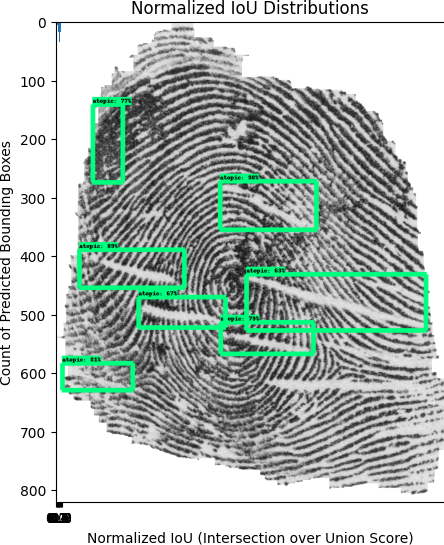
\includegraphics[width=120px]{obrazky-figures/atopic_eczema_FP_00183.png}
    \caption{Predikce atopického ekzému}
    \label{fig:predikce}
  \end{minipage}
  \hspace{0.5cm}
  \begin{minipage}[b]{0.5\linewidth}
    \centering
    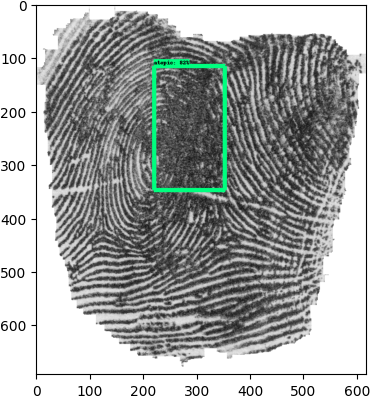
\includegraphics[width=120px]{obrazky-figures/atopic_eczema_FP_00193.png}
    \caption{Predikce atopického ekzému}
  \end{minipage}
\end{figure}

\begin{figure}[!htbp]
  \begin{minipage}[b]{0.5\linewidth}
    \centering
    \includegraphics[width=120px]{obrazky-figures/dys_SG11_1.png}
    \caption{Predikce dyshidrózy}
  \end{minipage}
  \hspace{0.5cm}
  \begin{minipage}[b]{0.5\linewidth}
    \centering
    \includegraphics[width=120px]{obrazky-figures/dys_SG12_5.png}
    \caption{Predikce dyshidrózy}
  \end{minipage}
\end{figure}

\begin{figure}[!htbp]
  \begin{minipage}[b]{0.5\linewidth}
    \centering
    \includegraphics[width=120px]{obrazky-figures/healthy_SG45_1.png}
    \caption{Model neučinil žádné predikce pro otisk prstu bez onemocnění}
  \end{minipage}
  \hspace{0.5cm}
  \begin{minipage}[b]{0.5\linewidth}
    \centering
    \includegraphics[width=120px]{obrazky-figures/healthy_SG78_5.png}
    \caption{Model neučinil žádné predikce pro otisk prstu bez onemocnění}
  \end{minipage}
\end{figure}

\begin{figure}[!htbp]
  \begin{minipage}[b]{0.5\linewidth}
    \centering
    \includegraphics[width=120px]{obrazky-figures/SG13_5.png}
    \caption{Predikce bradavic}
  \end{minipage}
  \hspace{0.5cm}
  \begin{minipage}[b]{0.5\linewidth}
    \centering
    \includegraphics[width=120px]{obrazky-figures/SG43_2.png}
    \caption{Predikce bradavic}
  \end{minipage}
\end{figure}

Při predikci se do souboru \verb=predictions.txt= zapisují informace o predikcích se skóre jistoty aspoň 50 \%. Níže je ukázka predikce pro snímek \ref{fig:predikce}:
\begin{verbatim}
FILE NAME: atopic_eczema_FP_00183.png
DETECTIONS: 
	CLASS: atopic eczema
	DETECTION SCORE: 98.44 %
	CLASS: atopic eczema
	DETECTION SCORE: 89.35 %
	CLASS: atopic eczema
	DETECTION SCORE: 80.77 %
	CLASS: atopic eczema
	DETECTION SCORE: 78.55 %
	CLASS: atopic eczema
	DETECTION SCORE: 76.88 %
	CLASS: atopic eczema
	DETECTION SCORE: 67.33 %
	CLASS: atopic eczema
	DETECTION SCORE: 62.71 %
\end{verbatim}








\chapter{Závěr}
Cílem tohoto semestrálního projektu bylo nastudovat literaturu týkající se zpracování otisků prstů, biometrie a konvolučních neuronových sítí. Je kladen důraz na popis onemocnění, které mohou oblast prstu postihnout a mnohdy ovlivnit proces rozpoznávání. Při studii konvolučních neuronových sítí jsem se zaměřila na výčet jejich architektur, až z důrazem na ty z nejnovějších. Modelů pro detekci objektů také existuje celá řada, opět byla snaha popsat u každého z modelů jakým způsobem případně vylepšuje jiná již existující řešení a na jakém je založen principu.

Pro následnou analýzu bylo vybráno několik architektur, se kterými bude dále experimentováno a bude probíhat jejich porovnání na základě různých hledisek. Budou provedeny experimenty i s parametry jednotlivých modelů. Následně byla oanotována část datasetu otisku prstů a jejich předzpracování s využitím morfologických operací. Také byl implementován kód pro načtení a konfiguraci modelu. Prvotní zkušební trénování pak bylo provedeno s modelem SSD MobileNet V2 FPNLite 320x320 s využítím klasifikace onemocnění atopického ekzému, bradavic a dyshidrózy. Nutno podotknout, že toto trénování proběhlo jen na části reálného datasetu atopického ekzému a pouze na syntetických snímcích s dalším onemocněním. Dataset tedy byl zatím pouze částečným a bude rozšířen i o snímky pacientů trpící těmito chorobami a bude experimentováno i s onemocněním psoriázy. Dále byla implementována metoda pro predikci a vizualizaci bounding boxů pro testovací dataset. Model bude muset být následně na testovacím datasetu ohodnocen - ať už z hlediska procentuálního překryvu, porovnání predikované a anotované třídy onemocnění nebo dalších technik.

Bude také potřebné vygenerovat více syntetických snímků s onemocněními, protože dataset reálných otisků prstů s onemocněními je velmi malým pro učení konvoluční neuronové sítě. Avšak bude potřeba otestovat model na snímcích z reálného datasetu, aby byl schopen model rozpoznávat a detekovat onemocnění otisků prstů reálných pacientů.
